\chapter{Overview}
\label{Overview}

\section{Introduction}
\label{Introduction}
Issues are an essential part of computer science and the development of software programs. For every software project there is a data set of issues, containing for example bugs, which disclose the problems of the current version of the program or features, which clarify new requirements for the software. \\ This is the reason for researchers to deal with issues or issue reports. Particularly with the analysis of these reports. The subject of software mining is concerned with the analysis of issues. Generally data mining means the systematic application of methods to a data set with the goal of identifying new patterns. Obviously, in the case of issue mining, this data set consists of issue reports. \\ Because of the importance of bugs and features there are several bug tracking systems to manage issue reports.
The critical problem for bug tracker miners is the different structure of the tracking systems. To mine issues, it is necessary to extract all the information of an issue. Therefore, bug tracker miners have a mining plan, which clarifies, what data can be found where. Now, the problem is, if you want to mine issues of different tracking systems, you have to create a mining plan for each system. \\ Furthermore, bug tracking systems are always developing and change their structure as part of a new version for example.
Than it is possible, that the origin mining plan doesn't work anymore or the extracted data are not reliable anymore. \\ Given these problems, a mining process could be very uncomfortable for issue miners and researchers. \\ So our aim is to improve the mining process in terms of an adaptive mining approach. We will try to automate the mining process. Given a bug tracking system, we want to create a method, that generates a mining plan that is specially geared to the structure of the respective tracking system. Finally we will be able to mine issues independent from a certain bug tracking system or a certain version. Our method will analyze the structure of the issue report and will submit a plan how to extract the data of the respective issue. \\ \\
In detail this means, we will create a data set of bug reports of a certain bug tracking system. When creating the issues we will assign the fields of the issue with predefined markers, so that we are able to recognize the data of the fields in later runs. After that, we will choose one report and access its HTML structure. Next, we will convert the HTML code to XML. With a depth-first search algorithm we will retrieve our markers and remember the respective path to it. We will frame this path as a XPATH expression that we can use to obtain our desired data by applying this expression to the XML code of an other bug report. Ideally we will be able to retrieve all our markers and to extract information of any bug report of this version of the bug tracking system. So the XPATH expression will be our mining plan respectively it denotes where we can find the information reports contain. \\ After obtaining our mining plan and the information of the issue, we will instantiate a new bug report with the corresponding information and put it in a new data base. \\ Given this expression, we can apply it to the other issues of our created data set for evaluation case. Furthermore our method will be able to generate an expression for an other version of the bug tracking system. In the best case we can extract all data the reports contain. For evaluation purposes we will test our method with three different bug tracking system and variable version of them. \\ \\ In summary, we try to simplify and automate the mining process concerning issue mining by developing an adaptive issue miner which uses data tracking and which is independent of the tracking system or its current version.



\section{Related Work}
\label{Related Work}
There are similar works concerning mining software repositories. A common method of data mining is the selection of information of bug reports to reference them to the original code. A.Schroeder et al. demonstrated two steps in their work 'If Your Bug Database Could Talk...' [1]. First they identified corrections with the message of the fix, which references to the concerning bug report (Fixed \# 3223 for example).\\ Second is, that they mapped bug reports to releases. The version field of the bug database lists the release for which the bug was reported. However they noted that the reliability respectively the trust level is very low. This work leads to the following question: In which parts of the code are the most bugs because of the complexity of the code? Therefore it is necessary to define a metric, that measures the complexity of the code. Such kind of metrics already exist ('Mining metrics to predict
component failures.'[2]), but this research doesn't give a definite answer. The conclusion is, that new metrics or a combination of existing metrics are required to measure the complexity better and more reliably. Consequently this approach of mining bug reports shows the potential of future research based on such bug data.\\ A similar approach chose J.Sliwerski, T.Zimmermann and A.Zeller in their paper 'When Do Changes Induce Fixes?' [3]. They analyzed CVS (Concurrent Versions System) archives for changes that lead to problems, indicated by fixes. They showed how to automatically locate fix-inducing changes by linking a version archive (such as CVS) to a bug database (such as BUGZILLA).\\ 
For the standardization of bug reports there already exists a software called MOZKITO, that realizes these tasks. MOZKITO (developed by Sascha Just and Kim Herzig) models bug reports in a way, that we can abstract all these trackers. So MOZKITO mines reports of different trackers, however not adaptive. Our goal is to develop a tool, that is able to mine bug reports adaptive. Concerning 'related work' there is nothing more to say, because, as seen, there are some earlier approaches in issue mining, but not in the way we are pursuing. 
\chapter{Concepts}
\label{Concepts}

\section{Problem}
\label{Problem}
The main problem of mining issues of different bug tracking systems is that they have distinct structure. One tracker uses components which are neglected by another. Or the tracking system uses various scales of classification. For example one bug tracker has five levels to classify the priority of an issue, the other uses only three levels to grade the priority. \\Up to now the common procedure was to mine manually with the help of a spider or a crawler (a computer program that gathers and categorizes information on a website). 
\\
 Hence, there is the next problem of manual issue mining, the changing API (application programming interface) of the issue tracker. Software programs like Redmine or BUGZILLA are always evolving and changing their interface. This fact is very unfavourable for non-adaptive issue miners, because such modifications often remain undetected and the mining software isn't working anymore or the data is not reliable anymore.\\
Furthermore there is no guarantee of the correctness of the mining process. \\ Our proposed solution is an adaptive miner. If we would be able to generate our miner automatically, we would create a robustness and independence against changes of the interface. Effectively themes like 'Tackling Interface Evolution in Issue Tracker for Software Mining' are close to our work. \\
Generally there are various possibilities to access data of bug trackers. Figure 0 shows a table with the currently most used bug tracking systems and the interface they provide.
The HTML surface, the XML part or the REST (Representational state transfer) API for example are possibilities to extract information. The latter is a method of communication between the user and the server of the bug tracking system. Similar possibilities are XML-RPC (Extensible Markup Language Remote Procedure Call), JSON-RPC (JavaScript Object Notation Remote Procedure Call) and SOAP (Simple Object Access Protocol). RPC means, by sending a HTTP request to a server, that calls a single method of a remote system, one return value is returned. In the case of XML-RPC the input and output format is XML, in the case of JSON-RPC the format is JSON. SOAP is the successor of XML-RPC.  \\
 For our case of an adaptive miner, we will decide for the first-mentioned, the HTML surface. All the mentioned capabilities change their  structure in consequence of the changing interface of the bug trackers.  Basically it doesn't matter which opportunity we will choose, because our conceptual approach is adaptive and independent. Nevertheless by using HTML front-end, we can guarantee that all relevant data are available.\\ Figure 1 shows the mentioned changing interface of bug tracking systems as Bugzilla. In version 4.4 in contrast to version 3.3.4 there are some small, but for bug miners very crucial modifications. For example in 3.3.4 the login fields are visible and the user is able to login directly. In 4.4 the user has to click the login button first, before being able to enter his username and password. These modifications of the HTML structure also influence the information miners want to extract. The location of data could change or, as in our example, an additional link could be necessary for the crawler to access the respective information.
\begin{table}
\centering
\begin{tabular}{|p{3cm}|p{10.5cm}|}
	\hline
	\textbf{Bugtracker} & \textbf{provided interface or access to data}  \\
	\hline
	\hline
	Bugzilla & can be accessed and modified by an XML-RPC or a JSON-RPC 	     Webservice interface \\
	\hline
	Mantis & with MantisConnect it can be accessed via SOAP \\
	\hline
	Roundup (SourceForge) & can only be accessed via the user interface, i.e. template files of HTML\\
	\hline
	Redmine & provides a REST API that supports XML and JSON format \\
	\hline
	Trac & provides a RSS feed, otherwise only the look can be accessed via HTML template and CSS files \\
	\hline
	JIRA & provides the Atlassian REST API \\
	\hline
\end{tabular}
\caption{The most used bug tracking systems and the interface they provide}
\label{tabelle interface}
\end{table} 

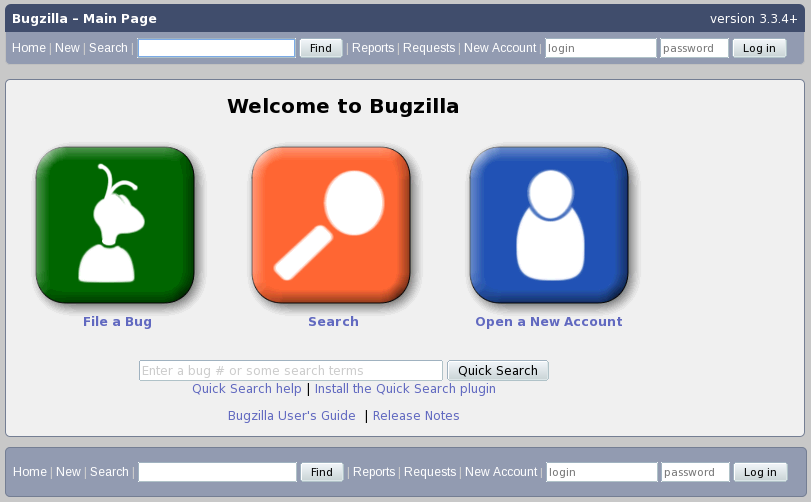
\includegraphics[width=1.0\textwidth]{bugzilla334} \\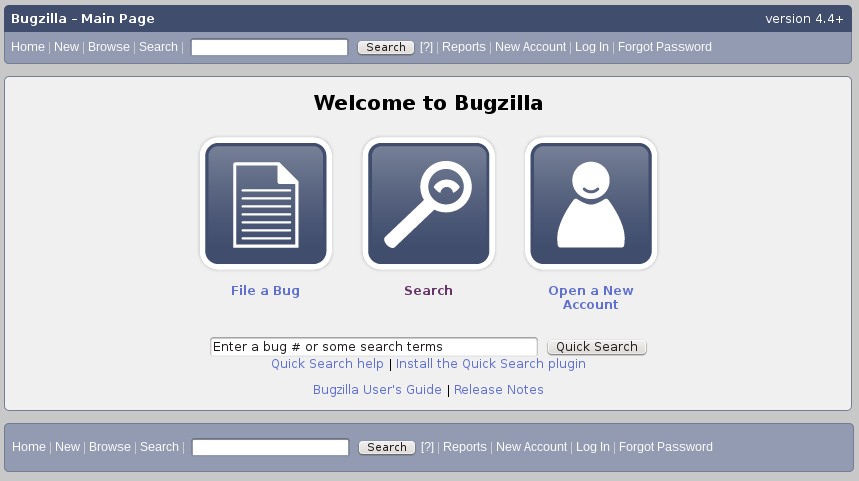
\includegraphics[width=1.0\textwidth]{bugzilla44}  \\\textbf{Figure 1}: \textit{As an example of the changing interface of a bug tracking system, the Bugzilla version 3.3.4 on top, at the bottom the version 4.4}
\newpage

\section{Contribution}
\label{Contribution}
First, we need a standardized view of bug reports. In the paper 'What Makes a Good Bug Report' 2007 [4], Nicolas Bettenburg et al. deal with the question, which information a good bug report would have to contain as well as in their paper 'Quality of Bug Reports in Eclipse' 2007 [5]. \\ Both papers conclude that information on steps to reproduce and stack traces are very important fields of a bug to be a bug report of high quality. The main problem, which resulted in the survey, that was conducted by Bettenburg et al., is the inaccuracy and incompleteness of bug reports. \\ Concerning our approach, this means that we need to define some standards to guarantee that we can compare issues of different bug tracking systems. We have to determine which fields of a bug report are important or significant. In other words, a feature-complete representation of issue reports is desirable. \\ \\ The second point is the reception of a benchmark. To develop our tool, we need to create a set of bug data, which represents the predefined standards in all facets. Partly we will construct this set manually, partly we will extract some existing bug reports from the MOZKITO database. Additionally, this is a basis on which other tools could test their mining results. \\ \\ The third point is our approach of adaptive mining. We will develop a tool, which analyzes the changing structure of reports in different bug tracking systems and generates a corresponding issue miner.  In other words, on the basis of a set of bug reports, our tool yields a mining plan, which states how to extract information of these reports to write them in a database. \\ Given such a tool, we could automatically create issue miner independent from the respective bug tracking systems. In other words, an on-the-fly production of bug tracker miners would be possible, given a way to deploy our created data set. The advantage of our tool, if the deployment would be defective, would be the recognition of this failure during the generating of the miner. The justification therefore is that we have our original data set. If we couldn't mine it with our tool, we would know that something goes wrong. We can always compare the mining results with our original data and determine if any data was mined wrong or if any data was lost. Furthermore modifications of the interface of bug tracking system would interest no longer. Such failures as shown in Figure 2 could also originate from changing interface of a bug tracker that non-adaptive miners don't recognize. \\ \\ 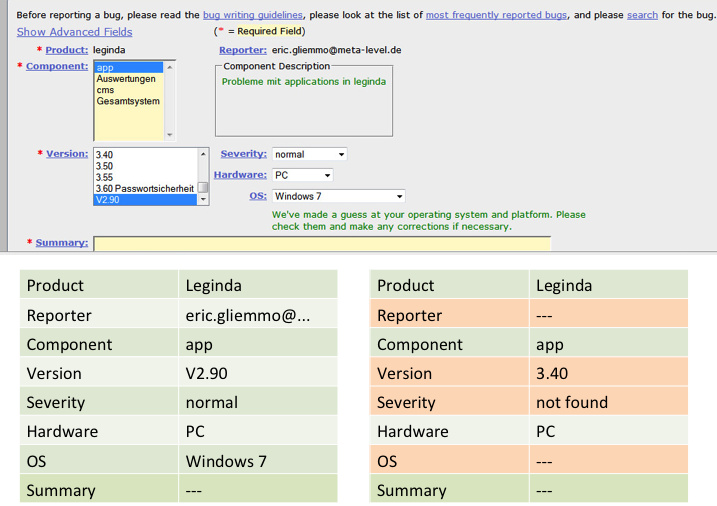
\includegraphics[width=1.0\textwidth]{Folie1.jpg}   \\\textbf{Figure 2}: \textit{On top, a bug report of Bugzilla , on the left the information of our original report and on the right the obtained data after a defective mining process}

\chapter{Method and Implementation}
\label{Method an Implementation}

\section{Methodology}
\label{Methodology}
At first we need a data set in the form of an issue report collection of different bug tracking systems. We will construct a large base of issues that we are able to test our tool on the basis of these data. Our data set has to satisfy several characteristics. For the test purposes at later, it is useful to create those data sets in three different bug tracking systems (BUGZILLA, Jira and SourceForge) and different versions of them to ensure that our tool doesn't work only in a particular case. As mentioned before, this collection will be feature-complete and represent our defined standards. \\ Next we access the HTML surface of our bug reports. HTML (HyperText Markup Language) is the main markup language for creating web pages and other information that can be displayed in a web browser. Tim Berners-Lee, the inventor of the World Wide Web, wrote a memo proposing an Internet-based hypertext system.[6] Berners-Lee specified HTML and wrote the browser and server software in late 1990. The first publicly available description of HTML was a document called "HTML Tags", first mentioned on the Internet by Berners-Lee in late 1991.[7] These days the standard version is HTML 4.01. Tools like Firebug (Figure 3) submit the HTML structure of a website. This structure can be easily converted to XML. Although the HTML and the XML appear very similar, this conversion is necessary. XML (Extensible Markup Language) is also a markup language that defines a set of rules for encoding documents in a format that is human-readable and machine-readable. It is defined in the XML 1.0 Specification produced by the W3C (World Wide Web Consortium), that was also engaged in the development of HTML 4. In contrast to HTML, whose primary purpose is to display data with focus on how the data look, XML is a dynamic language whose primary purpose is the transport and storage of data. That is the reason of our conversion, because we are interested in the containing data of the webpage and not in the design.\\ \\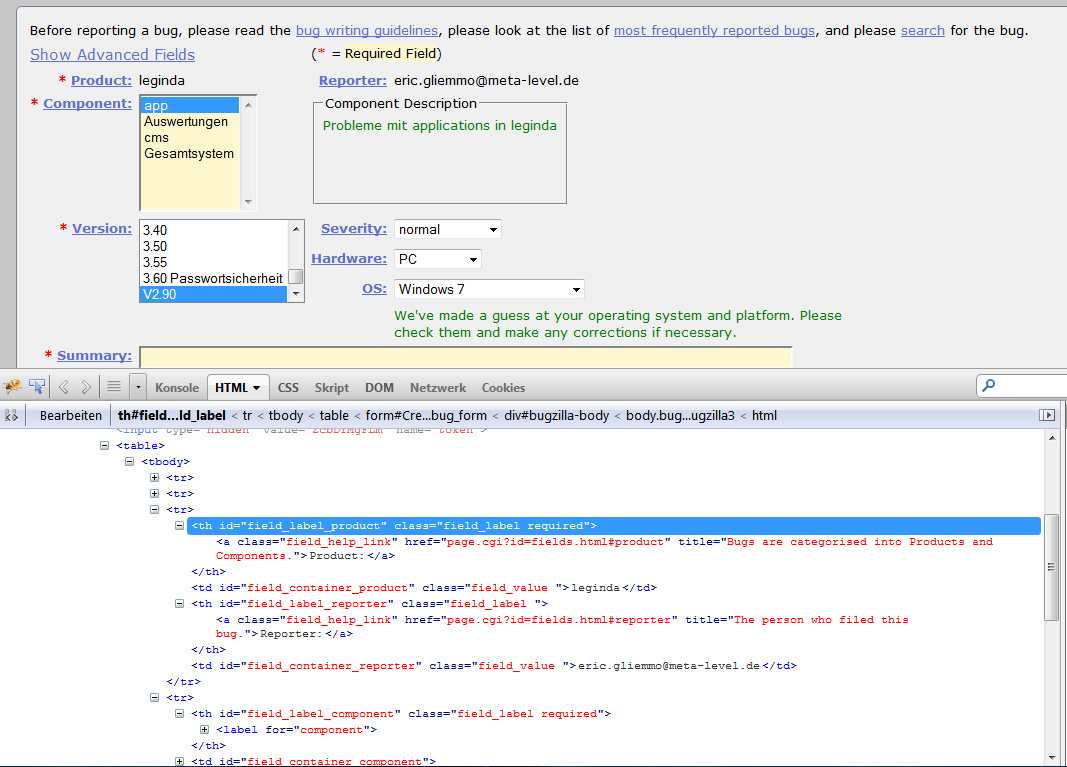
\includegraphics[width=1.0\textwidth]{Screenshot_bugzilla_html2.jpg}  \\\textbf{Figure 3}: \textit{On the top, a standard Bugzilla bug report in creation, below the HTML code of this report, extracted by Firebug}  \\ \\ However, at first glance, the syntax of both languages seems similar. With the use of HTML/XML, we can guarantee the completeness of the data of the website, in contrast to REST, XML-RPC or SOAP, in which this completeness is not secured. A reason therefore is, that HTML is the interface of the biggest target group respectively of the end-user. REST API, XML-RPC or SOAP aren't used by the ordinary user, so they aren't very well maintained and at the most not complete. They are often used only for tools with special assignments. For example the bug tracker MantisBT provides, apart from the HTML surface, SOAP as interface. Therefore the user has to use MantisConnect, a PHP web service that is built on top of Mantis API, that provides an easy way to connect to MantisBT via SOAP.   \\ The next step will be the use of a marker to retrieve our required information. In the XML code of the bug reports we will assign the important fields with markers. In this context the expression 'field' means an information field in a bug report or an issue. For example the priority or the description are such 'fields'. Every field gets a unique sequence of letters, by which we will be able to identify the field and will have a reference to the associated bug report. This marker is important concerning the crawler or spider in later runs. \\After that we put these adapted bug reports in the bug tracking systems mentioned before. Then the crawler or the spider comes to the use. A Web crawler starts with a list of URLs to visit. In our case, this is the URL of the concerning bug report in the bug tracking system. As the crawler visits these URLs, it identifies all the hyperlinks in the page and adds them to the list of URLs to visit next. In a bug report, these are additional information fields or attachments for example that are located on additional sites. Crawlers can validate hyperlinks and HTML code. So if we encounter one of our markers, we have to memorize where we found this marker respectively the associated field. That means that we have to create a mapping that clarifies which field or marker can be found where. So our abortive goal is to obtain a mining plan, that gives an instruction where we can retrieve our desired information. \\  Finally we have got a tool that submits, given some bug reports of a certain bug tracking system, a mining plan to find and select the information of the original bug report and yields these information back for example in the form of database records. 

\section{Preconditions}
\label{Preconditions}

\subsection{Adaption of a benchmark}
First we have to model issue reports with MOZKITO. 
++marker++
++marker in felder in die man was eintragen kann++
++bei auswahl feldern...mehrere reports die sich nur dort unterscheiden++
 


\subsection{Deployment of modified reports}
The first bug tracking system, we use to create a data set is JIRA. JIRA is a proprietary issue tracking product that is developed by Atlassian since 2002. The current version is JIRA v6.2, released 25 February 2014. [8] Our data set is created with version v6.0.7.

\section{Retrieving markers}
\label{Retrieving markers}

\subsection{Access the HTML structure}
The first obstacle of the plan is to access the HTML structure of a representative issue report. We need a possibility to handle the HTML code of the website and to work with it. For this purpose we will mainly deal with JDOM2. JDOM2 is the successor of JDOM and generally it is an open source Java-based document object model for XML and it is useful to manipulate XML code. It is a very common library to deal with XML in Java. Developed by Jason Hunter and Brett McLaughlin starting in March 2000, JDOM integrates "Simple API for XML" (SAX) and supports XPath, that is necessary for our mining plan in later runs. \\ So we have to find a way to convert the HTML code of the website to XML. This part TagSoup will realize. TagSoup is a SAX-compliant parser written in Java that, instead of parsing well-formed or valid XML, parses HTML as it is found in the web. So TagSoup supplies the parsed XML code of our issue report. By providing a SAX interface, it allows standard XML tools to be applied, such as we will do with JDOM2. \\ In fact this means, given the URL of an issue report we will apply TagSoup and Saxbuilder (part of the JDOM2 Sax library) to receive a JDOM2 Document with XML structure. The JDOM API represents a XML document with tree structure and grants access to the single components of the tree structure. Apart from the reading of the document with JDOM2 one is able to manipulate parts of the tree structure and the write back of the structure in the document. \\ \hrule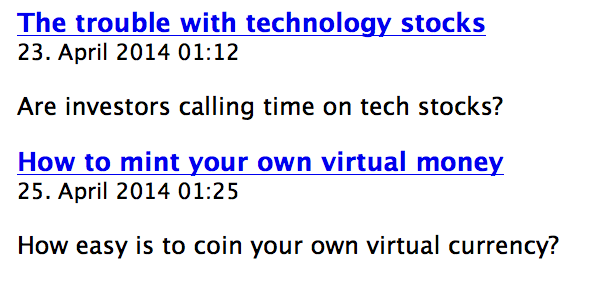
\includegraphics[width=1.0\textwidth]{website_ausschnitt.png} \\\textbf{Figure X}: \textit{An excerpt of a test website of BBC \\ (http://feeds.bbci.co.uk/news/technology/rss.xml?edition=int) with some information. Based on this data one can get an impression how TagSoup and JDOM2 work.}  \\ \\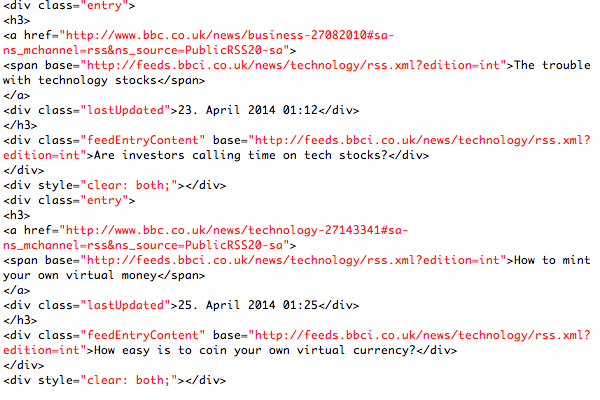
\includegraphics[width=\textwidth]{html_ausschnitt.png} \\ \hrule 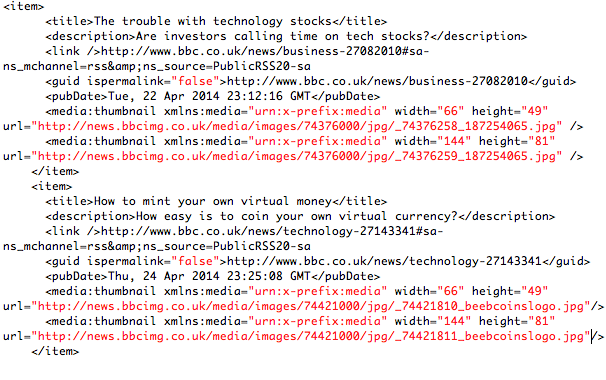
\includegraphics[width=1.0\textwidth]{xml_ausschnitt.png}  \\\textbf{Figure Y}: \textit{On the top, the HTML code of Figure X, extracted with Firebug, below the output of the JDOM2 document after applying TagSoup and Saxbuilder to the HTML code of the website}  \\ \\ \newpage With a simple, but comparable example one can illustrate how the conversion operates. Figure X shows a sample website containing some information comparable with the data of an issue report. In this form, the content is presented on the webpage. On the top of Figure Y, the HTML code of Figure X is located, extracted with Firebug. To deal with these information in Java it is useful to convert this code to XML. After applying TagSoup and Saxbuilder we obtain the JDOM2 document as mentioned before. The structure and information of this document is at the bottom of figure Y.\\ Obviously we obtain a typical XML document with tree structure. The advantage is, that with the JDOM2 library we can operate on this document for example to search for our markers. 


\subsection{Search in XML}
At first some words about XML and its structure. The Extensible Markup Language (XML) is a markup language for the representation of structured data in the form of text files. Every XML file has a logical structure that corresponds to a tree structure and therefore it is organized hierarchic.
\\ \\ 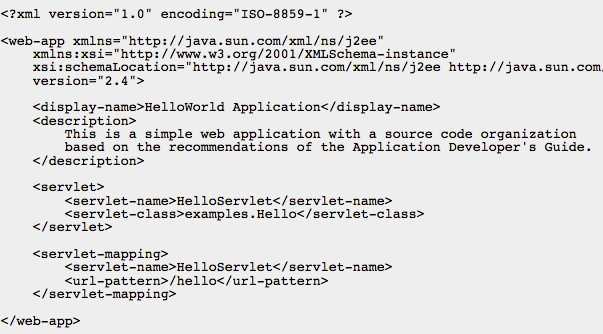
\includegraphics[width=1.0\textwidth]{xml_sample.png}  \\\textbf{Figure Z}: \textit{The tree structure of a simple XML document example}  \\ \\  Figure Z shows a standard XML document one can see this typical tree structure. The first line is the so called prologue, where the version of the XML is indicated. The part "encoding" is optional and an attribute of the prologue. Generally we deal with elements. An element consists of a tag and a content. We consider the example in figure Z. The line  $"<display-name>HelloWorld Application</display-name>"$ is such an element. $"<display-name>"$ ist the start tag of the element, $"HelloWorld Application"$ the content of the element and $"</display-name>"$ the end tag of the element. \\ Elements always have to be nested correctly. The start tag of an element contains the name of the element and optionally some attributes (for example the "encoding" in the prologue).[9] If we have a further element in the content of the origin element, we speak about a child element respectively a parent element. In figure Z for example the element $"web-app"$ is the parent element of $"display-name"$.\\ As mentioned before, we deal with a JDOM2 document with XML structure. So we have a root element (the element, that has no parent element) and child elements. In the case of JDOM2 library we will say nodes instead of elements.\\ Given the obtained JDOM2 document, we have to search for our markers and ideally remember the path to them. To simplify the algorithm we will only search for one marker. If found, we will remember the path to it and search the next one.  \\




\begin{algorithm}
\caption{SearchForMarker algorithm}\label{euclid}
\begin{algorithmic}[1]
\Procedure{$search\_for\_marker$}{$node$ $n$}\Comment{n is the root element}
\State $p\gets$ list of predecessors
\If{$p.size \neq depth$}
\State $p.add (n)$
\Else
\State $p.removelast$
\State $p.add (n)$
\EndIf

\For{$(x=0$,  $ x\le $ number of childs of $n$, $x$++$)$}
\If{child of $n$ has no children}
\If{text of $n$ contains marker}
\State finalpath $\gets p$
\State break
\EndIf

\Else 
\State$search\_for\_marker$ (child of $n$)
\EndIf
\EndFor
\EndProcedure
\end{algorithmic}
\end{algorithm}

Algortihm 1 shows the pseudocode of the algorithm we used to find the marker. With the input of a node $n$, the algorithm uses depth-first search to retrieve the marker. $p$ is the list of predecessors. Given, that we know the current $depth$ of our search, we save all parent nodes up to $n$ of our current node in the list of predecessors. In every recursive call of the procedure we check, if the size of the predecessor list is not equal to the depth. In the case $depth > p.size$, that means we are in a new plane of the tree structure and have to add our current to the list of predecessors. \\ If $depth = p.size$, we don't have a new plane and before adding the current node to the predecessor list, we have to delete the last one of it. \\ After that, in the for-loop we consider the children of node $n$. If the child $x$ of $n$ doesn't have any children, we test if the text of this node contains the marker we are looking for. If we found it, the predecessor list corresponds to the final path of the desired information. If the child $x$ of $n$ of the for loop has any children we call the procedure $search\_for\_marker$ with $x$ instead of $n$. \\ \\
So finally, if we found a marker, the $search\_for\_marker$ procedure yields a list with all the nodes of the XML document that are required to access the marker respectively the information of the corresponding node.


\section{Generating a mining plan}
\label{Generating a mining plan}
Next step is to develop a method, which we are able to apply this obtained list to an issue report of the same bug tracking system as the origin report. That means, given the list, we need a possibility to access information of a XML document. To extract information of a bug report, we will convert the HTML code of its website again and as in 3.3.1 we will deal with an JDOM2 document with XML structure. \\ The most obvious solution is to work with XPath. XPath, the XML Path Language, defined by the World Wide Web Consortium (W3C), is a query language for XML documents. Based on a tree representation of the XML document, the XPath language provides the possibility to navigate around the tree and select nodes. [10] \\
Ideally Xpath has been adopted by JDOM2, so that we can work with Xpath using the converted XML documents. Additionally we require Jaxen. Jaxen is an open source XPath library written in Java and it is adaptable to object models such as JDOM2. \\ After all we can use the XpathFactory. Given a XPath expression as a string this XPathFactory is able to generate a XPath object. With the help of another method of the XPath library we can evaluate this XPath object to the JDOM2 document of the concerning issue report. Finally this method provides the node, which contains the desired information respectively the marker in the origin issue report. \\ So we are able to access the content of a node, given a XPath expression as a string.
Therefore we have a small method, thats input is the predecessor list of 3.3 and the output is the corresponding XPath expression in the form a string.
\\ \\ 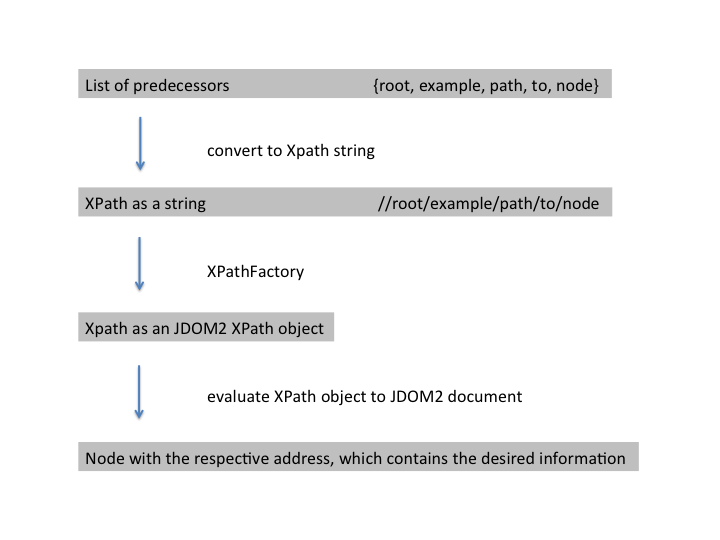
\includegraphics[width=1.0\textwidth]{list_to_xpath.png}  \\\textbf{Figure W}: \textit{The conversion of the predecessor list to a XPath expression which yields the desired node of the JDOM2 document}  \\ \\  

\chapter{Evaluation and Analysis}
\label{Evaluation and Analysis}
After developing our tool, we can test its correctness by applying it to our benchmark set. We will choose a set of random bug reports of our dataset and put them into three different bug tracking systems (BUGZILLA, Jira and SourceForge) and different version of these trackers. Then we will apply our tool to these bug reports and will compare the submitted results with our original data. If we get nearly the same information concerning the data sets after applying our tool, we can say that it is a good adaptive miner. \\ \\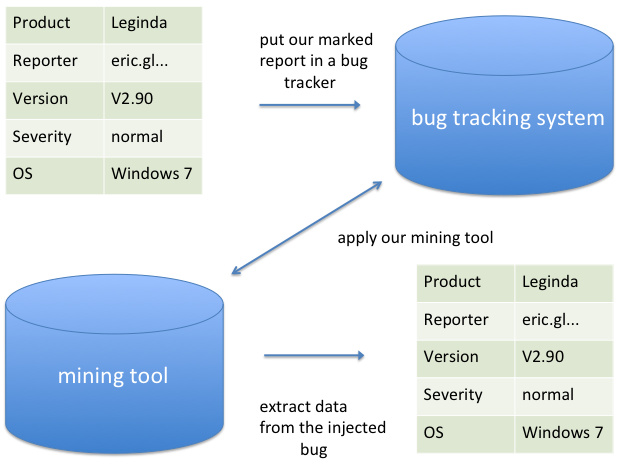
\includegraphics[width=1.0\textwidth]{Folie2.jpg}  \\\textbf{Figure 4}: \textit{A mining process of our tool without any loss of information.}  \\ \\
Figure 4 shows an optimal mining process. Ensuing from a bug report of our database equipped with our markers, we put this report in a bug tracking system, apply our mining tool and compare the result with our original bug report. We can attest ideal work to our tool if we obtain the same information as result, such as we put it in the bug tracking system. \\ Following problems could appear: On the one hand it is possible that we won't retrieve all information of the original reports. How to handle this problem? Or what could be the reason of this loss of data? Maybe our markers are not precise enough or the crawler does not work as planned. \\ On the other hand, what does it mean, if only two of three bug tracking systems yield good statistics concerning our evaluation of applying the tool?
\chapter{Conclusion}
\label{Conclusion}

\section{Summary}
\label{Summary}

\section{Future Work}
\label{Future Work}

%%%%%%%%%%%%%%%%%%%%%%%%%%%%%%%%%%%%%%%%%%%%%%%%%%%%%%%%%%%%%%%%%%%%%%%%%%%%%%%%%%%%%%%%%%%%%%%%%%%%%%%%%%%%%%%%%%%%%%%%%%%%%%%%%%%%%%%%%%%%%%%%%%%%%%%%%%%%%%%%%%%%%%%%%%%%%%%%%%%%%%%%%%%%%%%%%%%%%%%%%%%%%%%%%%%%%%%%%%%%%%%%%%%%%%%%
